

\chapter[Environmental Impacts of Lake Depletion]{Environmental Impacts of Lake Depletion}
\label{cp:environmental-impact}

\vspace{.935em}

The depletion of the Aral Sea has resulted in profound and far-reaching environmental consequences, transforming the previously flourishing ecosystem into a barren and inhospitable landscape. The extensive loss of water from the lake, driven by Soviet irrigation practices, has left a devastating legacy.

\section{Exposed Lakebed and Desertification}
As the water levels of the Aral Sea plummeted, vast stretches of the former lakebed became exposed, giving rise to dry, salt-encrusted terrain highly susceptible to erosion and toxic dust dispersion (\autoref{fig:exposed-lakebed}). What was once a vital aquatic ecosystem quickly became a desert, with salt and toxic residues left behind. The exposed lakebed, now known as the Aralkum Desert (\autoref{fig:aralkum-desert}), spans thousands of square kilometers and is a direct result of the lake’s shrinking. This transformation has not only altered the physical landscape but also contributed to the release of hazardous chemicals, such as pesticides, fertilizers, and heavy metals, into the environment \autocite{chen_dust}. These substances, once trapped in the lake water, have been carried by wind and dust storms across the region, further deteriorating the environment.

\begin{figure}[htpb]
    \centering
\fbox{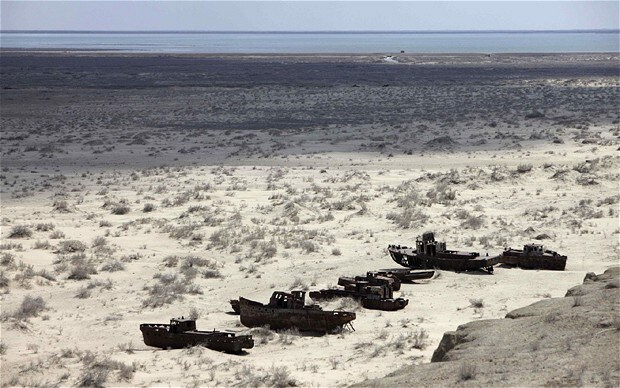
\includegraphics[width=0.7\linewidth]{Figures/The exposed lakebed.png}}
    \caption{The exposed lakebed}
    \label{fig:exposed-lakebed}
\end{figure}

\begin{figure}
    \centering
    \fbox{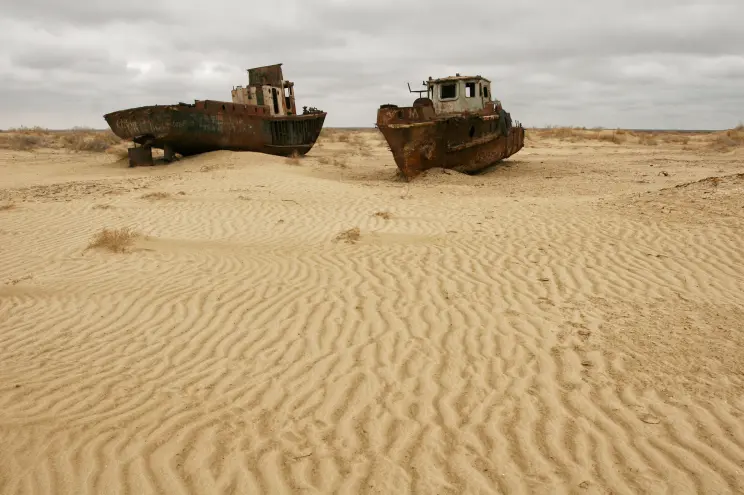
\includegraphics[width=0.7\linewidth]{Figures/Araklum Desert.png}}
    \caption{The Aralkum Desert}
    \label{fig:aralkum-desert}
\end{figure}

\section{Microclimate Disruptions}
The disappearance of the Aral Sea has also led to significant changes in the local climate. The lake had previously played a critical role in moderating the temperature of the region, creating a stabilizing effect on the surrounding microclimate. As the lake's surface area shrank, the region experienced more extreme weather conditions \autocite{narbayep_aral}. Summers became hotter, and winters colder, due to the loss of the lake's ability to absorb and release heat. In addition, precipitation levels began to decline, exacerbating the already arid conditions. These changes in climate have not only disrupted the natural environment but also negatively impacted the agricultural productivity of the surrounding areas \autocite{huseynli_aralcatastrophe}. 

\section{Biodiversity and Habitat Loss}
The dramatic ecological transformation of the Aral Sea has resulted in a profound loss of biodiversity and critical habitats. Once home to 24 native fish species, the lake experienced a sharp increase in salinity—from approximately 10 $g/L$ to over 100 $g/L$ in some regions—caused by the diversion of inflowing rivers for irrigation \autocite{schettler_hydrochemical}. This rendered the aquatic environment uninhabitable for most freshwater species, leading to the complete collapse of the fish population by the late 1990s (\autoref{fig:salinity-rise}) \autocite{gleick_araldeath}\autocite{aladin_zoocenosis_2019}. \autoref{cp:aral-wildlife} contains few such endangered or extinct fish species endemic to the Aral Region.

\begin{figure}
    \centering
    \fbox{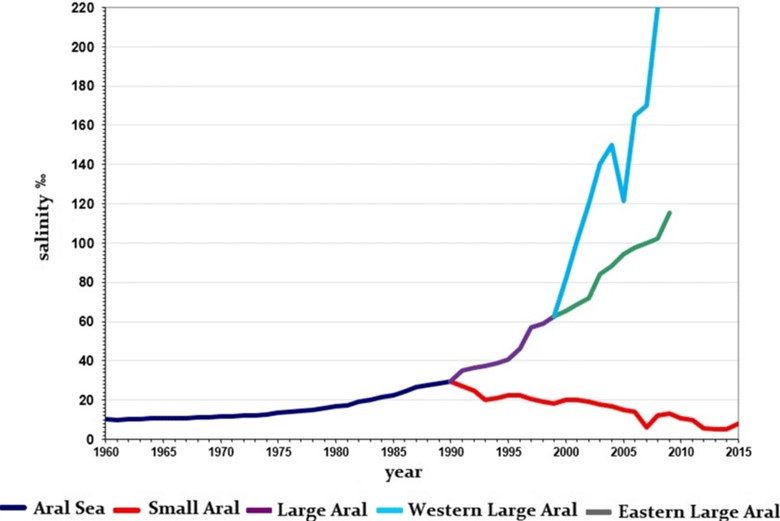
\includegraphics[width=0.8\linewidth]{Figures/Salinity rise.png}}
    \caption{Salinity rise in Aral}
    \label{fig:salinity-rise}
\end{figure}

Simultaneously, the shrinking shoreline of the Aral Sea led to the disappearance of extensive wetlands that had once bordered the lake and served as vital habitats for a wide variety of migratory bird species \autocite{joger2012fauna}. These wetlands provided essential breeding and feeding grounds for ducks, swans, pelicans, cormorants, and many other bird species (refer to \autoref{cp:aral-birds}) migrating through Central Asia. As these ecosystems disappeared, countless migratory birds were forced to abandon the region, struggling to find alternative habitats. This disruption triggered a severe decline in both regional and migratory biodiversity, with species such as muskrats and deer, which had depended on the wetlands, also becoming increasingly scarce \autocite{unesco2000vision}. This dual collapse of aquatic and avian life highlights the extensive ecological damage caused by the desiccation of the Aral Sea.
